\documentclass[type=master]{thuthesis}
% 选项:
%   type=[bachelor|master|doctor|postdoctor], % 必选
%   secret,                                   % 可选
%   pifootnote,                               % 可选(建议打开)
%   openany|openright,                        % 可选,基本不用
%   arial,                                    % 可选,基本不用
%   arialtoc,                                 % 可选,基本不用
%   arialtitle                                % 可选,基本不用

% 所有其它可能用到的包都统一放到这里了,可以根据自己的实际添加或者删除。
\usepackage{thuthesis}

% 定义所有的图片文件在 figures 子目录下
\graphicspath{{figures/}}

% 可以在这里修改配置文件中的定义。导言区可以使用中文。
% \def\myname{薛瑞尼}

\begin{document}
	
	%%% 封面部分
	\frontmatter
	\thusetup{
	%******************************
	% 注意:
	%   1. 配置里面不要出现空行
	%   2. 不需要的配置信息可以删除
	%******************************
	%
	%=====
	% 秘级
	%=====
	secretlevel={秘密},
	secretyear={10},
	%
	%=========
	% 中文信息
	%=========
	ctitle={绳驱超冗余连续型柔性臂的运动规划研究},
	cdegree={工学硕士},
	cdepartment={自动化系},
	cmajor={控制科学与工程},
	cauthor={于行尧},
	csupervisor={王学谦},
	%  cassosupervisor={陈文光教授}, % 副指导老师
	%  ccosupervisor={某某某教授}, % 联合指导老师
	% 日期自动使用当前时间,若需指定按如下方式修改:
	% cdate={超新星纪元},
	%
	% 博士后专有部分
	cfirstdiscipline={计算机科学与技术},
	cseconddiscipline={系统结构},
	postdoctordate={2009年7月——2011年7月},
	id={编号}, % 可以留空: id={},
	udc={UDC}, % 可以留空
	catalognumber={分类号}, % 可以留空
	%
	%=========
	% 英文信息
	%=========
	etitle={Motion Planning for Cable-driven Hyper-redundant Continuum Manipulator},
	% 这块比较复杂,需要分情况讨论:
	% 1. 学术型硕士
	%    edegree:必须为Master of Arts或Master of Science(注意大小写)
	%             “哲学、文学、历史学、法学、教育学、艺术学门类,公共管理学科
	%              填写Master of Arts,其它填写Master of Science”
	%    emajor:“获得一级学科授权的学科填写一级学科名称,其它填写二级学科名称”
	% 2. 专业型硕士
	%    edegree:“填写专业学位英文名称全称”
	%    emajor:“工程硕士填写工程领域,其它专业学位不填写此项”
	% 3. 学术型博士
	%    edegree:Doctor of Philosophy(注意大小写)
	%    emajor:“获得一级学科授权的学科填写一级学科名称,其它填写二级学科名称”
	% 4. 专业型博士
	%    edegree:“填写专业学位英文名称全称”
	%    emajor:不填写此项
	edegree={Master of Science},
	emajor={Control Science and Engineering},
	eauthor={Yu Xingyao},
	esupervisor={Wang Xueqian},
	%  eassosupervisor={Chen Wenguang},
	% 日期自动生成,若需指定按如下方式修改:
	% edate={December, 2005}
	%
	% 关键词用“英文逗号”分割
	ckeywords={关键词, 英文逗号},
	ekeywords={key, word}
}

% 定义中英文摘要和关键字
\begin{cabstract}
	论文的摘要是对论文研究内容和成果的高度概括。摘要应对论文所研究的问题及其研究目
	的进行描述,对研究方法和过程进行简单介绍,对研究成果和所得结论进行概括。摘要应
	具有独立性和自明性,其内容应包含与论文全文同等量的主要信息。使读者即使不阅读全
	文,通过摘要就能了解论文的总体内容和主要成果。
	
	论文摘要的书写应力求精确、简明。切忌写成对论文书写内容进行提要的形式,尤其要避
	免“第 1 章……;第 2 章……;……”这种或类似的陈述方式。
	
	本文介绍清华大学论文模板 \thuthesis{} 的使用方法。本模板符合学校的本科、硕士、
	博士论文格式要求。
	
	本文的创新点主要有:
	\begin{itemize}
		\item 用例子来解释模板的使用方法;
		\item 用废话来填充无关紧要的部分;
		\item 一边学习摸索一边编写新代码。
	\end{itemize}
	
	关键词是为了文献标引工作、用以表示全文主要内容信息的单词或术语。关键词不超过 5
	个,每个关键词中间用分号分隔。(模板作者注:关键词分隔符不用考虑,模板会自动处
	理。英文关键词同理。)
\end{cabstract}

% 如果习惯关键字跟在摘要文字后面,可以用直接命令来设置,如下:
% \ckeywords{\TeX, \LaTeX, CJK, 模板, 论文}

\begin{eabstract}
	An abstract of a dissertation is a summary and extraction of research work
	and contributions. Included in an abstract should be description of research
	topic and research objective, brief introduction to methodology and research
	process, and summarization of conclusion and contributions of the
	research. An abstract should be characterized by independence and clarity and
	carry identical information with the dissertation. It should be such that the
	general idea and major contributions of the dissertation are conveyed without
	reading the dissertation.
	
	An abstract should be concise and to the point. It is a misunderstanding to
	make an abstract an outline of the dissertation and words ``the first
	chapter'', ``the second chapter'' and the like should be avoided in the
	abstract.
	
	Key words are terms used in a dissertation for indexing, reflecting core
	information of the dissertation. An abstract may contain a maximum of 5 key
	words, with semi-colons used in between to separate one another.
\end{eabstract}

% \ekeywords{\TeX, \LaTeX, CJK, template, thesis}

	% 如果使用授权说明扫描页,将可选参数中指定为扫描得到的 PDF 文件名,例如:
	% \makecover[scan-auth.pdf]
	\makecover
	
	%% 目录
	\tableofcontents
	
	%%% 符号对照表
	%\input{data/denotation}
	
	
	%%% 正文部分
	\mainmatter
	\chapter{课题的来源背景以及研究意义}
\section{课题来源}

课题来源于。。。。。拟针对绳索驱动的新型超冗余连续型柔性臂在复杂工作环境下进行探测等任务,进行系统的运动学建模,样机的设计及调试,并进一步研究探索针对此类柔性臂的运动学规划及避障算法。
\section{研究背景及意义}

随着经济的发展和社会的进步,机器人的应用领域不断拓展,应用环境也愈发复杂。以工业机器人为代表的传统刚性机械臂在结构化的工作环境下的程序化操作得到了广泛应用,但刚性机械臂在非结构环境(例如废墟、复杂管道等)下的局限性正日益显露。在传统工业机器人中,电机、传动机构等被放置于关节臂杆中,不仅增大了关节的质量,还加大了关节尺寸;另外,受制于质量和体积的限制,具有长而粗臂杆的这类刚性机械臂的自由度往往较少,其运动的灵活性进一步恶化,难以完成狭小环境下的各类作业要求。为了解决传统机器人在复杂环境下操作所面临的问题,许多研究人员将目光投向了具有更多运动自由度更好弯曲特性的连续型机器人的研究中。

连续型机械臂受自然界中象鼻等生物体结构启发,一般由弹性物体作为支撑,将许多模块化关节串联而成,或者直接用完整无间断的弹性材料作为机械臂本体,因而具有超高冗余度甚至理论上无限多自由度。这种结构形式使得连续型机械臂具有良好的运动灵活性和柔顺性,因而特别适合于狭小空间下的避障作业。图\ref{fig:compare_tra_con}显示了传统刚性臂与连续型机械臂在狭小环境中作业能力的差异。可以看出,具有超高冗余度的连续型机械臂具有更好的弯曲特性和障碍穿越能力。
\begin{figure}[!htbp]
	\centering
	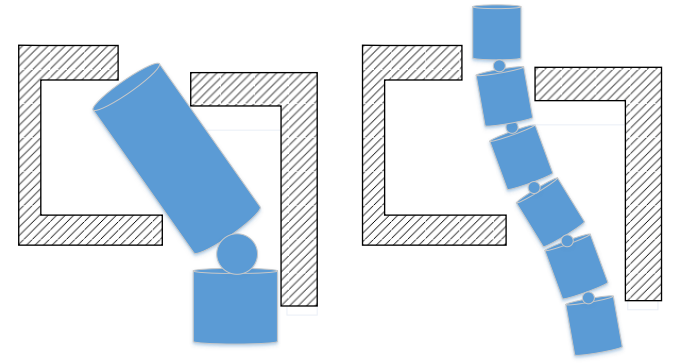
\includegraphics[width=.75\textwidth]{figures/compare_tra_con.png}
	\caption{传统刚性机械臂与连续型机械臂在狭小空间中的作业能力对比}
	\label{fig:compare_tra_con}
\end{figure}

连续型柔性臂的灵活性、柔顺性使得其在非结构复杂环境中具有广阔的应用前景。在航空航天领域中,连续型柔性臂可以穿越航天器的桁架结构和组件间隙,深入到结构内部进行探测、在轨维修等任务\cite{xu_modified_2017};在工业生产领域,可以通过孔洞等深入结构内部进行钻孔、焊接等工作(如图\ref{fig:app_airplane}和图\ref{fig:app_pipeline});在危险环境中,可以进入到狭小缝隙中进行结构的探伤和检修(如图\ref{fig:app_nuclear});可用于地震后废墟内生命迹象检测(如图\ref{fig:app_debri});还可用于外科手术中对体内空腔结构的检查和微创手术等(如图\ref{fig:app_surgery})。
\begin{figure}[h]
	\centering%
	\subcaptionbox{飞机舱内钻孔\label{fig:app_airplane}}
	{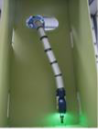
\includegraphics[height=4cm]{figures/app_airplane.png}}%
	\hspace{1em}%
	\subcaptionbox{复杂管道中焊接\label{fig:app_pipeline}}
	{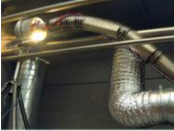
\includegraphics[height=4cm]{figures/app_pipeline.png}}
	\hspace{1em}%
	\subcaptionbox{核电站设备检修\label{fig:app_nuclear}}
	{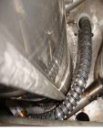
\includegraphics[height=4cm]{figures/app_nuclear.png}}
	\\
	\vspace{1em}
	\subcaptionbox{地震灾害救援\label{fig:app_debri}}
	{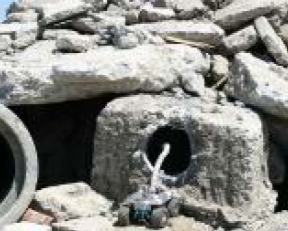
\includegraphics[height=4cm]{figures/app_debri.png}}
	\hspace{1em}%
	\subcaptionbox{外科手术\label{fig:app_surgery}}
	{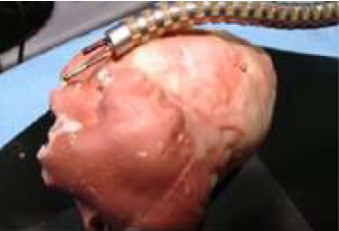
\includegraphics[height=4cm]{figures/app_surgery.png}}
	\caption{连续型机械臂在各种复杂环境中的应用}
	\label{fig:apps}
\end{figure}

从驱动方式上看,连续型机器人可分为腱驱动式、同心圆管式和其他新型机构驱动等三类。绳索作为腱的一种,采用其作为驱动传动机构,具有以下优点:首先,通过柔性绳索传动,原本位于关节连接处的电机、控制电路、减速装置等可以迁移到根部基座上,实现驱动机构和执行机构的分离,从而使得电机控制电路等远离外界复杂环境的不利影响,并且能够显著减小机械臂的体积和质量;其次,关节质量和体积的减小意味着在整体质量和体积的约束下,机械臂可以增加更多的关节模块,从而使得机械臂具有更多的运动自由度,也就具有更强的运动灵活性和避障能力;再者,绳索驱动的连续型机械臂相比于其他种类的连续型机器人,对材料工艺等要求较低,结构也比较简单,更容易进行原理样机的设计和制作。

综上所述,为了应对新的复杂环境对机器人提出的新挑战,有必要对连续型机器人展开研究,采用绳索驱动,可以减小机械臂重量和体积,组装具有超冗余度的柔性臂,并探索其在非结构环境中运动规划方法。


	\chapter{连续型机械臂的研究现状}
	\section{连续型机械臂的发展历程}
%	介绍,应用场景、历史发展、连续型机器人的概念。

受自然界象鼻、章鱼腕足、藤蔓等柔性组织或结构的启发,很多研究团队针对连续型机器人展开了深入广泛的研究。与传统的由刚性臂杆及刚性关节构成的机器人相比, 连续型机器人具有很强的灵活性和内在的柔顺性,因此在航空航天\cite{walker_robot_2013}、微创手术(MIS) \cite{conrad_interleaved_2017,gilbert_elastic_2016} 等领域获得了越来越多研究者的关注。
 
连续型机器人的概念首先由Robinson等人提出\cite{robinson_continuum_1999},他们认为连续型机器人是能够通过弹性变形沿长度方向连续弯曲,产生光滑的曲线来实现运动的一类新型机器人。宽泛的讲,连续型机器人的决定性特征是具有能够连续变化的支撑结构,并且这种结构富有柔顺性。因此,由小段刚性模块和整体弹性支撑构成的超冗余机器人,其在一定程度上具有连续型柔性臂的特征。但从严格意义上讲,这类超冗余串联机器人并不属于连续型机器人,因为它们只能产生近似连续曲率的空间曲线。一些学者为了严格划分,将这类模块化结构组成的超冗余机器人称为“连续风格(continuum-style)”机器人\cite{walker_continuous_2013}和“类连续型(pseudocontinuum robot)机器人”\cite{burgner-kahrs_continuum_2015}等。
%	实际上,连续型机器人具有无限多自由度,而上述类连续型机器人则在刚性结构下限制了自由度的个数,从而将无限自由度的超冗余机器人归化为具有有限自由度的超冗余机器人。

对于连续变形的机器人的研究始于上世纪60年代。Tensor Arm被认为是第一次见于文献的连续型机器人原型\cite{anderson_tensor_1967}。它是一种绳驱的超冗余机器人(图\ref{fig:tensor_arm}),其输入与变形之间的关系相较于传统刚性机器人十分复杂。经历了约十年的冷寂期后,90年代前后,对于连续型机器人的建模问题取得了突破。Chirikjian将超冗余机器人的构型近似为严格意义上的连续型机器人,利用连续空间曲线建立了运动学和动力学\cite{chirikjian_hyper-redundant_1994}
\begin{figure}
	\centering
	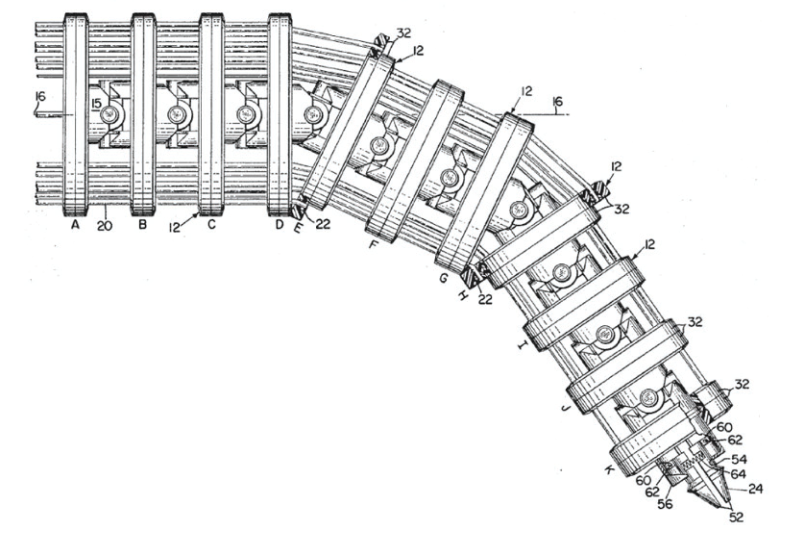
\includegraphics[width=.75\textwidth]{figures/tensor_arm.png}
	\caption{Tensor Arm机器人}
	\label{fig:tensor_arm}
\end{figure}
Ivanescu等建立了电流变液驱动的动力学模型并用滑膜方法和Bang-Bang方法进行了控制\cite{ivanescu_variable_1995}。本世纪前后,连续型机器人的研究取得了长远的进步。Clemson大学的Walker教授带领的研究团队对连续型机器人进行了广泛深入的研究,并研制了多款物理样机\cite{hannan_analysis_2001,gravagne_manipulability_2002,mcmahan_field_2006,walker_robot_2013,tonapi_next_2014,tonapi_novel_2015}。
新型连续型机器人的设计\cite{yigit_design_2017,conrad_interleaved_2017,qi_novel_2016}、运动学和动力学\cite{chikhaoui_kinematics_2016,godage_dynamics_2016}、控制和规划\cite{chikhaoui_kinematics_2016}等各方面的研究方兴未艾。

\section{连续型机器人的分类}
%	腱驱动、同心管、新型驱动(人造肌肉)与变刚度、软体机器人 。问题:轴向压缩回程间隙振动
%	传统的刚性结构机器人由于结构上不会发生柔性变形,因此可以通过有限个关节驱动其在三维空间运动;而连续型机器人的连续型弯曲变形

连续型机器人本质上可以是一种欠驱动机器人,其具有无限多自由度的弯曲变形仅能依靠有限多驱动源驱动,因此为了实现连续可控的弯曲变形,需要通过设计合适的机械结构和驱动方式进行对空间弯曲进行约束。
从驱动方式上看,连续型机器人一般可以分为腱驱动连续型机器人(Tendon-driven Continuum Manipulator)、同心圆管连续型机器人(Concentric Tube Continuum Manipulator)和新型驱动(如人工肌肉)机器人。
%	另外需要说明的是,软体机器人也是连续型机器人的一种\cite{robinson_continuum_1999},它们多采用腱驱动\cite{renda_3d_2012,renda_dynamic_2014}和新型驱动方式\cite{rus_design_2015,marchese_dynamics_2016,marchese_design_2016}。
\subsection{腱驱动机器人}
由于结构的限制,连续型机器人往往无法像传统机器人一样,将驱动单元直接与关节连接,而是通过绳子或弹性棒等柔性材料与位于机器人外部的驱动单元连接,远程驱动机器人弯曲变形,这类机器人属于腱驱动机器人。
%	这是一种外部驱动方式。
 
腱驱动连续型机器人的一般结构形式是由弹性支撑和均布于其四周的腱(绳子或弹性杆等),以及位于基座部位的驱动单元组成。机器人一般分为多节,每一节的末端有一组腱与之固连,驱动单元的驱动力经由腱传递到每一节的末端,从而使弹性支撑产生连续弯曲变形。图\ref{fig:tendril}中的Tendril机器人是典型的腱驱动机器人,它使用一系列可压缩弹簧作为弹性支撑,每个电机驱动一对绳子控制一个方向的弯曲\cite{mehling_minimally_2006}。
\begin{figure}[!htbp]
	\centering
	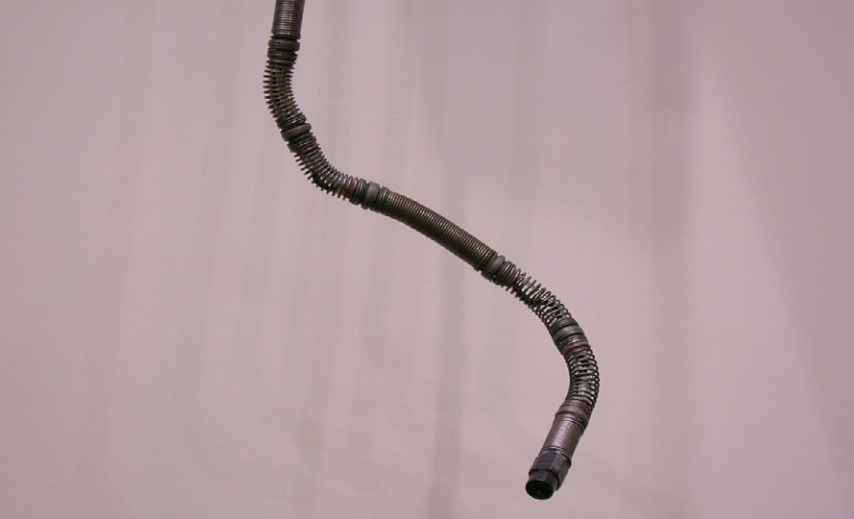
\includegraphics[width=.75\textwidth]{figures/tendril.png}
	\caption{Tendril机器人,腱驱动}
	\label{fig:tendril}
\end{figure}
 
这类机器人存在的主要问题有:
\begin{enumerate}
	\item 绳子的驱动力会同时会使得弹簧等可压缩弹性材料产生轴向压缩,导致弯曲变形和轴向压缩产生耦合,轴向压缩会导致弹性支撑刚度变大,柔顺性变差;
	\item 多节连续型机器人的驱动腱往往是利用过孔限制与机体一起变形,即后一节的驱动腱需要随前一节的变形而改变长度,造成了节间驱动的耦合,驱动误差会逐节累积放大,末端控制精度不高。
	\item 在往复运动过程中,绳子等单向施力的腱可能出现松弛\cite{hannan_kinematics_2003}和回程间隙\cite{bardou_control_2010}等问题。
\end{enumerate}
%	产生弯曲的另外,由于驱动每一节弹簧的绳子需要穿过其之前的部分,导致驱动误差(绳子长度的变化)逐节累积放大,造成了控制上产生很大的误差。
 
解决上述问题的思路有:
\begin{enumerate}
	\item 选择柔性不可压缩材料作为弹性支撑\cite{gravagne_large_2003,liu_development_2016,suh_design_2015,gao_workspace_2015}。例如MCMahan等设计了采用气压软管作为弹性支撑的Air-Octor机器人,通过气压变化控制弹性支撑的伸长和收缩,通过绳子控制弯曲\cite{mcmahan_design_2005}。Qi等设计了一种采用双层平面弹簧串联组成的连续型机器人,柔顺性分析表明,这种设计能够使得伸缩和弯曲解耦\cite{qi_novel_2014,qi_novel_2016};
	\item 
	将腱放置在机体外面,驱动器与力的作用点之间仅有腱连接,或实时估计变形对节间耦合造成的影响,进而补偿\cite{tonapi_novel_2015};
	\item 
	可以通过增加弹簧补偿机构\cite{hannan_kinematics_2003}或采取每根腱用一个电机驱动\cite{shang_design_2012}的方式解决松弛和回程间隙等问题。另外,将弹性棒同时作为腱和弹性支撑,既能解决了绳子作为腱会产生的问题,同时可以增加控制上的灵活性\cite{rone_mechanics_2014}。
	
\end{enumerate}
%	为了解决上述问题,一般选择柔性不可压缩材料作为弹性支撑\cite{gravagne_large_2003,liu_development_2016,suh_design_2015,gao_workspace_2015}。MCMahan等则设计了采用气压软管作为弹性支撑的Air-Octor机器人,通过气压变化控制弹性支撑的伸长和收缩,通过绳子控制弯曲\cite{mcmahan_design_2005}。Qi等设计了一种采用双层平面弹簧串联组成的连续型机器人,柔顺性分析表明,这种设计能够使得伸缩和弯曲解耦\cite{qi_novel_2014,qi_novel_2016}。

腱驱动连续型机器人的优点是设计思路比较简单,负载能力较强,因而得到了较广泛的研究,并出现了商业产品(OC机器人)。
%	但由于往往采用多节设计,腱可能出现松弛\cite{hannan_kinematics_2003}和回程间隙\cite{bardou_control_2010}的问题。这些问题可以通过增加弹簧补偿机构\cite{hannan_kinematics_2003}或采取每根腱用一个电机驱动\cite{shang_design_2012}的方式进行处理。Rone等将弹性棒同时作为腱和弹性支撑,解决了绳子作为腱会产生的问题\cite{rone_mechanics_2014}


\subsection{同心圆管机器人}
同心圆管机器人是另一种采用外部驱动的连续型机器人,一般是由多个具有高弹性材料(如Ni-Ti合金等)制作的同心圆管相互嵌套构成。
%	同心圆管之间可以相互滑动和绕同心轴旋转。
\begin{figure}[!htbp]
	\centering
	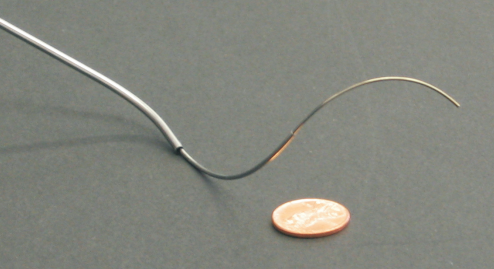
\includegraphics[width=.75\textwidth]{figures/ctm.png}
	\caption{同心圆管机器人\cite{webster_toward_2006}}
	\label{fig:ctm}
\end{figure}
 
同心圆管机器人可以实现长度上的伸缩和圆管绕同心轴的扭转,但受结构尺寸的限制,弯曲一般无法直接驱动。为了解决这个问题,一般将同心圆管进行预变形处理,这样具有初始曲率的内圆管在外圆管中滑动时,会在外圆管的的限制下发生弯曲变形\cite{sears_steerable_2006,webster_toward_2006,bergeles_concentric_2015,butler_robotic_2012}。

同心圆管机器人的机械设计上很简洁,并且由于主体部分只有相互嵌套的圆管,长细比可以非常大,常用于微创手术\cite{hendrick_hand-held_2015}等领域。该类机器人的缺点则包括载荷较小,弯曲无法直接驱动、工作空间较小等。
\subsection{具有新型驱动的连续型机器人}
与腱驱动机器人一样,同心圆管机器人的内圆管的弯曲变形与外圆管的形状参数有关,外圆管的变形直接对内圆管产生影响,因此采用外部驱动的连续机器人一般会存在节间耦合的问题,为了解决这一问题,许多采用内部驱动的新型驱动机器人被设计出来。
%	以上两种连续型机器人在采用多节设计是,后一节和前一节的驱动之间是相互耦合的。对于腱驱动来说,后一节的腱往往要穿过前一节的结构,前一节的结构变化就会使得在驱动后一节时要补偿掉前一节的该变量;对于同心圆管机器人来说,内圆管的弯曲变形是与外圆管的形状参数直接联系的,外圆管的变形直接对内圆管产生影响。为了解决这两种外部驱动存在的节间耦合的问题,研究这们设计了许多在节内部进行驱动的新型驱动机器人。
 
这类连续型机器人的驱动主要有气压(液压)人工肌肉、形状记忆合金\cite{ayvali_towards_2012-1}等。
气压(液压)人工肌肉是在气压或液压的作用下改变长度,进而驱动连接的端点发生伸缩、弯曲变形\cite{pritts_design_2004,guglielmino_octopus_2010}。OctArm(图\ref{fig:octarm})采用人工液压肌肉作为每一端点的驱动,成功进行了对不同形状目标的抓取和水下实验\cite{mcmahan_field_2006,trivedi_geometrically_2008}。
德国Festo公司的BHA机器人用波纹管是一种液压驱动的连续型机器人,它通过改变驱动波纹管的液压来说实现弯曲、伸缩\cite{falkenhahn_dynamic_2017}。Chikhaui等在同心圆管机器人的基础上添加了电活性聚合物(Electro-Active Polymers,EAP)作为控制器,从而实现对弯曲变形的主动控制\cite{chikhaoui_kinematics_2016}。
\begin{figure}[!htbp]
	\centering
	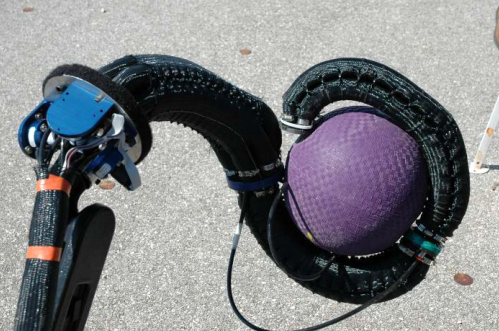
\includegraphics[width=.75\textwidth]{figures/octarm.png}
	\caption{OCtArm抓取物体实验\cite{mcmahan_field_2006}}
	\label{fig:octarm}
\end{figure}

内部驱动的连续型机器人能够直接驱动实现机器人的伸缩、弯曲、扭转变形,避免了其他两种连续型机器人的节间耦合,液压人工肌肉驱动等还能够产生较大的负载。这类机器人的缺点则是可能需要液压源和气压源,复杂的管道和阀门设计以及较高的加工装配精度。

\section{运动学}
和传统机器人运动学一样,连续型机器人的运动学一般也由三个空间之间的映射组成,即驱动空间、构型空间和任务空间。驱动空间与构型空间之间构成驱动运动参数(例如绳子长度变化)与连续型机器人形状参数(弯曲角度、弯曲方位)的映射关系,这一映射关系与机器人的设计有关,例如驱动方式不同,驱动空间参数一般也会不同;构型空间与任务空间构成形状参数与末端位姿之间的映射关系,这一映射与机器人设计无关\cite{webster_design_2010}。另一方面,运动学模型由结构参数直接决定的传统机器人不同,连续型机器人具有无限多自由度和内在的柔顺性,其结构参数在运动过程中是不断变化的,这种复杂性使得运动学建模方法成为了连续型机器人研究中的核心问题之一。
 
上述三类连续型机器人中,同心圆管机器人可以直接驱动嵌套圆管的滑动和伸长,不需要建立驱动空间与构型空间之间的映射。而对于采用腱驱动人工肌肉等新型驱动的连续型机器人,根据构型参数描述的空间变形采用几何学方法即可建立驱动空间与构型空间的映射关系\cite{jones_kinematics_2006,jones_practical_2006,webster_design_2010}。由于驱动空间与机器人的设计有关,因此目前并未有统一的建模方法。
%	下面主要针对构型空间与任务空间之间的映射关系进行介绍。
 
%	传统机器人的运动学模型由结构参数直接决定,而连续型机器人由于具有无限多自由度和内在的柔顺性,其结构参数在运动过程中是不断变化的,这种复杂性使得运动学建模方法成为了连续型机器人研究中的核心问题之一。
为了建立构型空间与任务空间的映射,一般采用几何的方法,通过对空间曲线的描述来建立二者之间的关系。在众多方法中,常曲率假设由于极大简化了运动学模型,因而在连续型机器人的建模中得到了广泛使用。
%	为了简化和近似描述连续型机器人的空间变形,一般假设机器人的形状具有常曲率。采用常曲率模型简化了运动学模型,易于实现多节的建模和逆运动学,在
%	同心圆管机器人可以直接驱动嵌套圆管的滑动和伸长,因此不需要建立驱动空间与构型空间之间的映射。而对于腱驱动机器人和人工肌肉等新型驱动机器人,根据构型参数描述的空间变形采用几何学方法即可建立驱动空间与构型空间的映射关系\cite{jones_kinematics_2006,jones_practical_2006,webster_design_2010}。
%	Tonapi等,采用实验数据建立变形与绳长变化的关系,对轴向压缩问题造成的误差进行了修正\cite{tonapi_novel_2015}.Camarillo等针对绳子松弛问题
%	采用优化的方法进行解决\cite{camarillo_configuration_2009}。
 
采用常曲率假设后,可以直接根据几何关系确定构型参数与机器人形状之间的关系\cite{bailly_modeling_2005,neppalli_design_2007}。还可以利用传统刚性机器人运动学建模所用的DH参数等工具。这种方法实际上是用离散的旋转和平移等效出连续型机器人上两点之间的位姿关系\cite{hannan_kinematics_2003,hannan_analysis_2001,walker_continuous_2013},对于平面连续型机器人,可以用旋转-平移-旋转三次操作来确定两点之间的位姿关系,对于空间运动,则可以用两次旋转一次平移和两次旋转进行确定\cite{hannan_kinematics_2003}。
 
虽然常曲率假设具有模型简单,计算量小的优点,但很多连续型机器人本质上无法产生常曲率的空间曲线。为了更精确的描述机器人的空间构型,需要考虑更为广泛的空间曲线表示方法。常用的方法有积分表示、模态函数等。积分表示是指表示出曲线上任一点切线的参数化坐标后,对其进行线积分以获得曲线上任一点的位置和空间指向\cite{chirikjian_hyper-redundant_1994,ivanescu_variable_1995}。模态函数则是用一系列基函数的线性组合来近似描述机器人的空间曲线,这类基函数包括三角函数\cite{chirikjian_modal_1994-1}、小波基函数\cite{gravagne_kinematics_2000}等。Godage等则直接用驱动空间参数的多项式对构型进行近似\cite{godage_shape_2011,godage_novel_2011,godage_dynamics_2016},从而之间建立了驱动空间与任务空间之间的映射关系。

 
另外,由于弹性体的变形和受力是紧密耦合的,因此在外力和扰动作用下,常曲率假设这种简单的几何假设可能不足以充分描述连续型机器人的运动学。Cosserat理论是对弹性介质在外力作用下变形的一个有力工具,利用Cosserat理论可以建立几何上比较精确地非常曲率运动学模型\cite{trivedi_geometrically_2008,jones_three_2009,rucker_geometrically_2010,mahvash_stiffness_2011,renda_general_2012}。但是这种模型计算上比较复杂,需要设计高效的计算方法才能够用于实时控制和模拟\cite{till_efficient_2015}。

%逆运动学?
一般来说,将上述方法建立的正运动学反解即可得到逆运动学\cite{sears_steerable_2006,camarillo_configuration_2009,neppalli_closed-form_2009},但由于连续型机器人具有的超冗余特性,即使采用常曲率假设进行简化也往往得不到解析解,需要采用数值计算方法\cite{jones_kinematics_2006,camarillo_mechanics_2008}。当机器人中存在非线性变形、未知干扰时,可以采用机器学习的方法学习逆运动学\cite{giorelli_feed-forward_2013,giorelli_neural_2015,rolf_efficient_2014,lakhal_hybrid_2016}。
%速度级运动学?


\section{动力学、控制和规划}
连续型机器人的动力学建模方法主要有牛顿-欧拉法\cite{khalil_dynamic_2007,kang_dynamic_2011}、拉格朗日方法\cite{mochiyama_kinematics_2003,godage_shape_2011,marchese_dynamics_2015,falkenhahn_dynamic_2015,godage_dynamics_2016}、集总参数法\cite{falkenhahn_dynamic_2015,falkenhahn_dynamic_2017,giri_three_2011,zheng_dynamic_2012}等。牛顿-欧拉法多用于模块化关节构成的连续风格的机器人,即有限自由度的机器人,而对于连续变形的具有无限自由度的机器人动力学建模来说,多采用拉格朗日方法。
%	与传统的刚性机器人不同,由于连续型机器人多由弹性材料组成,需要考虑材料变形中储存的弹性势能。
集总参数法多用于软体机器人和新型驱动机器人,是将弹性体等效为一个弹簧阻尼系统进行处理。连续型机器人的动力学模型与传统刚性机器人的区别主要是需要考虑弹性材料变形给结构参数带来的变化以及引入的弹性势能等。
 
%运动学、动力学、力、规划
由于连续型机器人难以像工业机器人等在关节处添加各种传感器,因此对其控制的研究大多是位置级。Qi等针对模型中存在不确定性,利用线性化后的状态空间模型建立了模糊控制器\cite{qi_kinematic_2016}。Marchese等设计了靠弹性材料局部膨胀实现弯曲的软体机器人的构型控制、正运动学算法等\cite{marchese_design_2016}。Yip等提出了一个任务空间的不依赖于模型的闭环控制器\cite{yip_model-less_2014},其思想是在线迭代估计机器人的雅克比矩阵。Chen等讨论了受限环境下基于传感器的位置引导控制方法\cite{chen_sensor-based_2009}。
%动力学
%	  
%	一般在建立连续型机器人的动力学模型后,会采用前馈控制对机器人的构型进行控制。
Falkenhahn等针对液压驱动的BHA机器人提出具有串联结构的前馈控制器\cite{falkenhahn_dynamic_2017}。Ivanescu等对非线性动力学解耦后采用滑膜控制策略对腱驱动连续型机器人进行了变形控制\cite{ivanescu_decoupled_2015}。Braganza等将神经网络作为前馈环节对OctArm进行动力学控制\cite{braganza_neural_2007}。
%力控
 
虽然连续型机器人具有柔顺性特点,特别适用于与环境存在交互的应用场合,但对这类机器人力柔顺的控制的研究还刚刚起步。
Bajo和Sim
aan提出了一种混合力位控制控制策略,并通过实验验证了该方法在连续型机器人与环境发生接触时的有效性\cite{bajo_hybrid_2016}。
%规划
%Chibani等提出了一个在约束环境下运动学构型的优化算法\cite{chibani_generating_2015}.
Goldman等用支持向量机估计标称模型中的非线性,设计了一种力柔顺策略\cite{goldman_compliant_2014}。Mahvash讨论了手术机器人的刚度控制,以实现末端指定力的输出\cite{mahvash_stiffness_2011}

	\chapter{主要研究内容}
\section{绳索驱动连续型柔性臂的运动学模型}
	连续型机器人的运动学由两部分组成,一是驱动空间与构型空间的映射;二是构型空间与工作空间之间的映射,如图\ref{fig:map}所示。对于绳索驱动的连续型机器人来说,驱动空间由驱动绳索的长度变化$\Delta l_i$构成,构型空间是指每个关节的弯曲角度,一般可以用弯曲方向$\phi_i$和弯曲角度描述$\theta_i$;工作空间则是指机械臂末端的位置$x,y,z$和指向。建立绳索驱动的连续型机器人的运动学,即是建立这三者之间的相互映射关系。
	\begin{figure}[h]
		\centering
		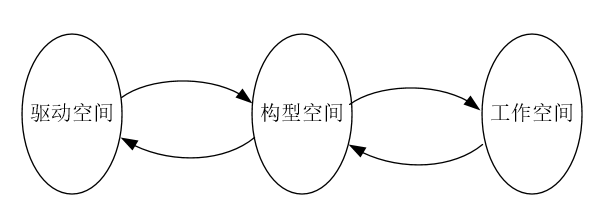
\includegraphics[height=4cm]{figures/map.png}
		\caption{连续型机器人的运动学组成}
		\label{fig:map}
	\end{figure}

	在研究这三类空间的映射关系时,一般先建立单个关节或单个臂段的运动学模型,然后利用链式法则推广成为整个机械臂的运动学模型。
	
	单个关节或臂段的驱动空间与构型空间之间的关系一般由几何关系建立。如图\ref{fig:single_joint}所示,位于单个关节之间的绳索长度可以等效成连接过孔的矢量长度$| \overrightarrow{B_i P_i}| $。由于圆盘上的过孔在各自的圆盘坐标系下的位置固定,因此在建立了两个圆盘坐标系($\{O x_{j-1} y_{j-1} z_{j-1}\}$ 和 $\{O x_{j} y_{j} z_{j}\}$)的坐标变换关系之后,即可得到绳索长度。
	\begin{figure}[h]
		\centering
		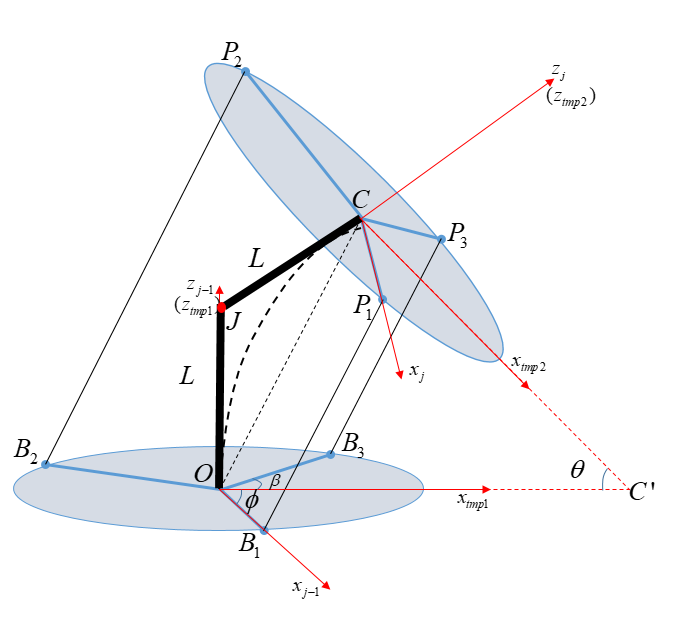
\includegraphics[height=7cm]{figures/single_joint.png}
		\caption{单个关节弯曲示意简图}
		\label{fig:single_joint}
	\end{figure}

	令$T_{j-1}^{j}$代表两个圆盘坐标系$\{O x_{j-1} y_{j-1} z_{j-1}\}$ 和 $\{O x_{j} y_{j} z_{j}\}$之间的齐次坐标变换,则绳索长度可以按照式\ref{eq:len}求解
	\begin{equation}
	| \overrightarrow{B_i P_i} | = \mathsf{C}_{\overrightarrow{OB_i}} - T_{j-1}^{j} \mathsf{C}_{\overrightarrow{C P_i}}  ||
	\label{eq:len}
	\end{equation}
	其中,$\mathsf{C}_{\cdot} $是$\cdot$在本体坐标系下的齐次坐标表示。
	
	虽然单个关节的驱动空间和构型空间之间的关系比较简单,但对于多个关节或臂段串联的机器人整体来说,这一映射关系可能会因为节间的耦合关系而变得复杂。远端臂段的驱动绳索往往要经由近端臂段过孔导引,因此近端臂段的弯曲变形会直接造成远端驱动绳索的长度变化,在计算远端的驱动参数时,应该补偿掉由于节间耦合带来的长度变化。
	
	构型空间与工作空间之间的关系由链式法则得到。对于具有$N$个关节或臂段的连续型机器人来说,其根部基座与末端位姿之间的齐次变换关系为:
	\begin{equation}
	T_{0}^{N} = \prod_{j=1}^{N} T_{j-1}^{j}
	\label{eq:chain}
	\end{equation}
	
	值得注意的是,在上述建立映射关系的过程中,所采用的都是几何上的关系,并未用到经典的D-H方法。因而在这种建模方法下,D-H方法的很多技巧和结论是很难直接运用的。受此影响,经典的Jacobian矩阵构造方法无法使用,需要另行推导简洁的雅可比矩阵构造方法。
	
	
	
	
\section{微分运动学模型的建立}
	得到机械臂的齐次变换之后,可以直接对变换矩阵进行求导并进行分离变量,以获得Jacobian矩阵\cite{hannan_kinematics_2003}。但这一非构造方法需要进行符号计算,并且计算量很大,限制了其应用。在建立运动学模型的过程中,我们采用的是几何关系,因此Jacobian矩阵应该也存在几何意义上的构造方法。
	
	对于图\ref{fig:single_joint}所示的由球铰连接的单个关节或臂段弯曲运动前后的齐次变换关系可以用旋量表示为:
	\begin{equation}
	T_{j-1, j} (\theta, \phi)= e^{\hat{\xi} \theta} T_{j-1, j}(\theta_0, \phi_0)
	\label{eq:ex_trans}
	\end{equation}
%	可以计算得到
%	\begin{equation}
%	e^{\hat{\xi} \theta} = T_{j-1, j} (\theta, \phi)T^{-1}_{j-1, j}(\theta_0, \phi_0)
%	\end{equation}
%	\begin{equation}
%	\omega = [-\sin\phi, \cos\phi, 0]^T
%	\label{eq:w}
%	\end{equation}
%	\begin{equation}
%	v = [-L\cos\phi, -L\sin\phi, 0]^T
%	\end{equation}
	进而可以得到空间速度如式\ref{eq:velocity}。
	\begin{equation}
	\begin{aligned}
	\hat{V}_{j-1,j}^{j-1} &= \dot{T}_{j-1,j}(\theta,\phi) {T}^{-1}_{j-1,j}(\theta,\phi)\\
	&=\frac{d}{dt}(e^{\hat{\xi} \theta}) T^{-1}_{j-1,j}(0,0) (T^{-1}_{j-1,j}(0,0))^{-1} (e^{\hat{\xi} \theta})^{-1}\\
	&=\frac{d}{dt}(e^{\hat{\xi} \theta})(e^{\hat{\xi} \theta})^{-1}
	\end{aligned}
	\label{eq:velocity}
	\end{equation}
	由于$\hat{\xi}$随弯曲方向变化,式\ref{eq:velocity}的简化需要借助于Lie Bracket工具。
	\begin{equation}
	\frac{d}{dt}(e^{\hat{\xi} \theta}) = dexp_{(\hat{\xi}\theta)} \frac{d(\hat{\xi}\theta)}{dt} e^{\hat{\xi} \theta}
	\label{eq:dexp}
	\end{equation}
	\begin{equation}
	dexp_{(\hat{\xi}\theta)} \frac{d(\hat{\xi}\theta)}{dt} = C + \frac{1}{2!}[A, C] + \frac{1}{3!}[A, [A, C]] + \cdots
	\label{eq:liebracket}
	\end{equation}
	其中,
	$$ [A, C] = AC-CA $$
	$$ A= \hat{\xi}\theta = \begin{bmatrix}
	\hat{\omega} & v \\
	\mathbf{0} & 0
	\end{bmatrix} \theta $$
	$$ C = \frac{d(\hat{\xi}\theta)}{dt}$$
	
	在得到单个关节的雅可比矩阵之后,则可以通过链式法则得到整个连续型机械臂的微分运动模型。
	

\section{运动学逆解及规划方法研究}
连续型柔性臂的逆解问题即是在给定期望位置后,计算每个关节臂段的弯曲角度和弯曲方向,进而利用构型空间与驱动空间之间的映射关系,得到绳索长度的变化。由于连续型柔性臂的高冗余度特点,位置级逆运动学求解难以解析获得,需要采取数值迭代等方法来解决。
\subsection{基于微分运动学的逆运动学求解}
基于微分运动学的逆运动学求解是借助于雅可比矩阵伪逆,在已知当前迭代位置$ \mathbf{p}_c $的情况下,利用位置误差$ d\mathbf{p} = \mathbf{p}_d -\mathbf{p}_c $得到构型参数的变化量$d\mathbf{q}$。经过不断的数值迭代,最终使得迭代位置于期望位置重合\cite{webster_closed-form_2009}。算法的流程图如\ref{fig:flowchart}所示。
\begin{figure}[!htpb]
	\centering
	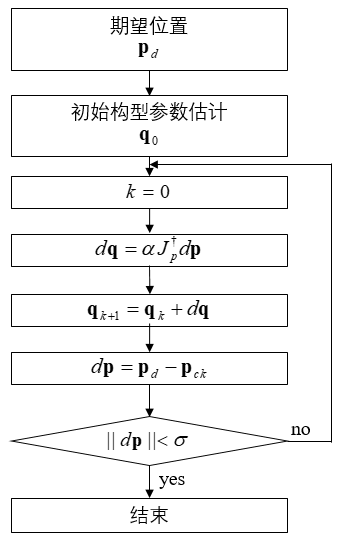
\includegraphics[width=5cm]{figures/flowchart.png}
	\caption{基于微分运动学的逆运动学求解流程图 }
	\label{fig:flowchart}
\end{figure}
\subsection{基于模态函数的逆运动学求解}
基于模态函数的逆解方法是由Chirikjian最早提出的\cite{chirikjian_obstacle_1990, chirikjian_geometric_1992}。被广泛应用于超冗余机械臂的逆运动学求解。这类方法的核心思想是用脊线刻画超冗余机械臂的宏观几何形状,进而将实际机械臂向这条脊线拟合,从而直接确定每一段关节所需的构型参数。脊线是分段连续的曲线,可以由给定的期望位置和模态函数经过迭代计算获得。采用这类方法进行连续型机械臂逆运动学求解的流程如图所示。
\begin{figure}[!htpb]
	\centering
	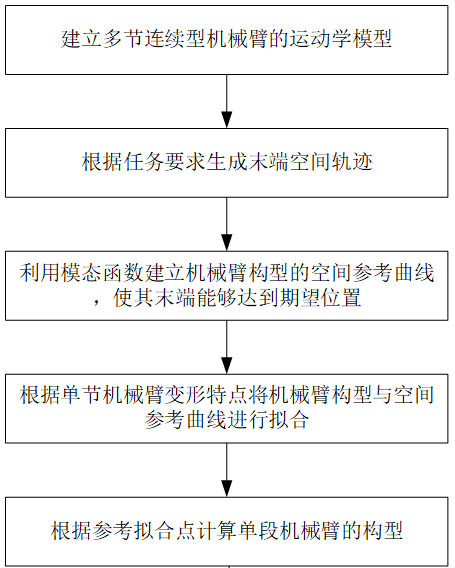
\includegraphics[width=6cm]{figures/flowchart_modal.png}
	\caption{基于模态函数的逆运动学求解流程图 }
	\label{fig:flowchart_modal}
\end{figure}
	\chapter{研究方案、预期成果及进度安排}

\section{研究方案与预期成果}
本毕业设计拟对绳索驱动超冗余连续型柔性臂的运动规划进行研究。首先建立连续型机器人的运动学模型,在此基础上探索其在复杂非结构化空间下的轨迹规划。通过研制物理样机,对运动学模型和逆解及规划算法进行验证。预期的成果有:
\begin{enumerate}
	\item 连续型机器人的位置级运动学模型。 
	
	结合物理样机,推导连续型机器人的完整运动学模型,建立驱动空间、构型空间和工作空间之间的映射关系,为后续的工作奠定基础;
	
	\item 球铰连接的连续型机械臂的微分运动学模型。
	
	借助旋量工具,推导具有球铰连接或柔性体连接结构的连续型机器人的微分运动学模型。建立Jacabian矩阵的构造方法,研究连续型机械臂的运动学奇异情况;
	
	\item 基于Jacobian矩阵伪逆的轨迹规划方法。
	
	利用Jacobian矩阵构造方法,研究基于伪逆的轨迹规划算法,通过仿真验证和样机实验进行验证;
	
	\item 基于模态函数的轨迹规划方法研究。
	
	采用脊线作为机器人宏观形状的刻画,提出基于脊线拟合的运动学逆解及规划算法,通过仿真实验和样机实验进行验证;
	
	\item 复杂空间中避障策略研究。
	
	在上述轨迹规划算法的基础上,研究连续型柔性臂在复杂非结构空间中的避障策略,使得其能够具备狭小空间中的作业能力,通过仿真实验和样机实验进行验证。
	
\end{enumerate}

\section{进度安排}
\begin{table}
	\centering
	\caption{毕业设计工作进度安排}
	\begin{tabular}{c|c}
		\toprule[1.5pt]
		时间 & 工作内容 \\
		\midrule		
		$\scriptsize{\sim}$2017.12.17 & 文献调研,物理样机的制作、装配和调试 \\
		2017.12.18 & 开题报告 \\
		2017.12.19 $\scriptsize{\sim}$ 2018.1.31 & 运动学模型的建立,运动学规划算法的仿真研究 \\
		2018.2.1 $\scriptsize{\sim}$ 2018.7.31 & 物理样机的进一步调试和实验 \\
		\bottomrule[1.5pt]
	\end{tabular}
\end{table}
	\chapter{关键难点及解决措施}
\section{研究过程中可能遇到的关键难点}
根据前期的文献调研,在研究过程中可能会遇到以下关键难点:
\begin{enumerate}
	\item 理论模型和实际物理模型不相符。
	
	在建立连续型柔性臂的运动学模型的过程中,为了简化,往往认为臂段按照常曲率进行弯曲。然而,臂段的实际弯曲形态的物理规律是十分复杂的,而且是与机械臂的受力紧密相关。在实际模型中,绳索经过过孔时产生的摩擦力、臂段的重力、绳索对过孔的压力等都会造成臂段弯曲形态背离常曲率假设,因此,理论模型和物理模型之间很可能出现偏差。
	
	\item 实验系统的运动参数测量。
	
	由于柔性臂的臂段是不断弯曲变化的,因此在理论模型存在偏差的情况下,无法直接根据驱动空间参数得到臂段的弯曲角度、末端位置等运动参数。柔性臂结构紧凑,难以在臂段上直接安装传感器,因此直接对实验系统的运动参数进行测量可能是比较困难的。
	
\end{enumerate}
\section{相应的解决措施}
为解决以上问题,拟采用以下解决措施:
\begin{enumerate}
	\item 通过样机实验获得数据,进而采用模型辨识的方法对理论模型进行修正。
	
	虽然实际样机的准确模型会非常复杂,但驱动空间、构型空间和工作空间之间的映射关系应该是固定的,可以在理论模型的基础上,采集实验数据,采用拟合或神经网络等方法模型进行修正;
	
	\item 采用外部非接触式测量。
	
	为了获得柔性臂弯曲之后的形状参数,可以借助深度相机等视觉测量设备,实现非接触式测量。
\end{enumerate}
	
	
	%%% 其它部分
	\backmatter
	
	%%% 本科生要这几个索引,研究生不要。选择性留下。
	%% 插图索引
	%\listoffigures
	%% 表格索引
	%\listoftables
	%% 公式索引
	%\listofequations
	
	
	%% 参考文献
	% 注意:至少需要引用一篇参考文献,否则下面两行可能引起编译错误。
	% 如果不需要参考文献,请将下面两行删除或注释掉。
	% 数字式引用
	\bibliographystyle{thuthesis-numeric}
	% 作者-年份式引用
	% \bibliographystyle{thuthesis-author-year}
	\bibliography{ref/ref2}
	
	
	%%% 致谢
	%\include{data/ack}
	
	%%% 附录
	%\begin{appendix}
	%\input{data/appendix01}
	%\end{appendix}
	
	%%% 个人简历
	%\include{data/resume}
	
	%%% 本科生进行格式审查是需要下面这个表格,答辩可能不需要。选择性留下。
	%% 综合论文训练记录表
	%\includepdf[pages=-]{scan-record.pdf}
\end{document}
